Les capteurs de température et d'humidité sont basés sur un protocole
MODBUS (non détaillé ici), codant les informations en binaire et les
envoyant via une liaison série.

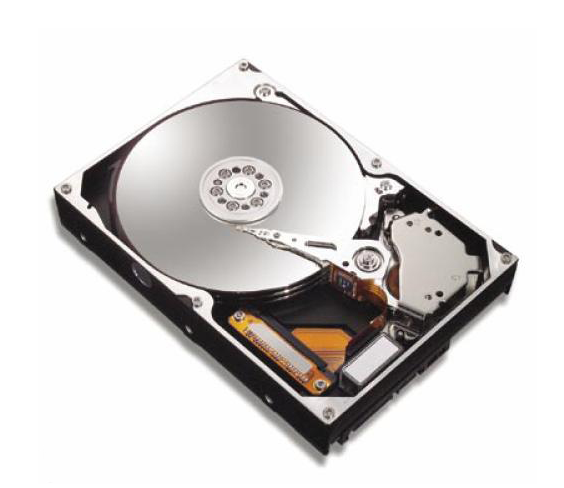
\includegraphics[width=1.70833in,height=1.14583in]{media/image2.emf}L'analyse
des trames envoyées qui suit permettra de décoder l'information et de la
recoder suivant la norme IEE754.

Le protocole Modbus permet à un matériel maître d'accéder jusqu'à 255
esclaves connectés sur un même bus. Chaque esclave se voit attribué une
adresse qui le différencie des autres esclaves connectés sur le bus.

Les transactions ne peuvent être qu'à l'initiative du maître et sont de
deux types :

\begin{itemize}
\item
  question / réponse~: 1 un seul esclave est adressé
\item
  broadcast / pas de réponse~: tous les esclaves sont adressé, mais ils
  ne doivent pas répondre
\end{itemize}

On ne détaillera qu'une trame \emph{\textbf{simplifiée}} constituée de
l'information des registres 5 et 6, et du contrôle~:

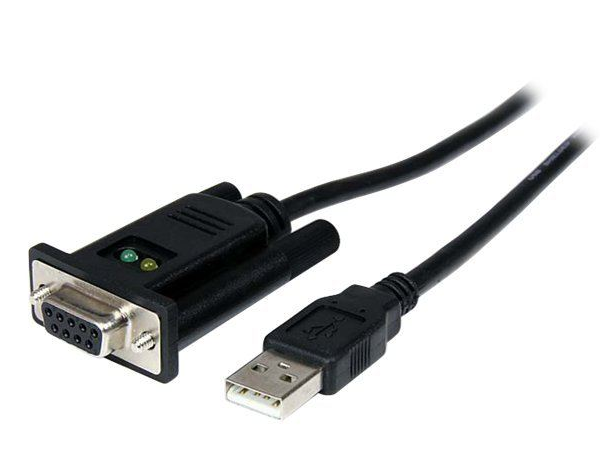
\includegraphics[width=1.26042in,height=1.47917in]{media/image3.jpeg}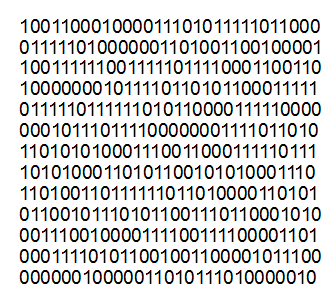
\includegraphics[width=6.40625in,height=1.71701in]{media/image4.png}

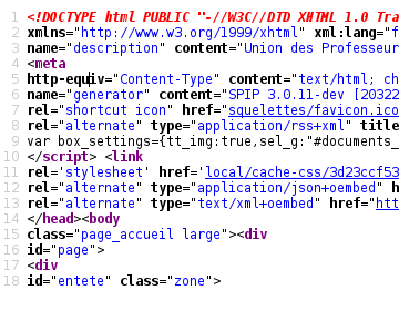
\includegraphics[width=3.01042in,height=0.69121in]{media/image5.png}

\textbf{Code contrôle} (8 bits)~: somme des \textbf{octets} envoyés
\emph{(extrait doc. Constructeur)}

Un exemple de trame (\emph{simplifiée}) transmise en réponse par le
capteur serait~:

\textbf{0000 0010 1000 1100 1111 1111 0111 0110 0000 0011}

Codage Humidité codage Température Checksum (contrôle)

Les données transmises sont donc~:

\begin{itemize}
\item
  16 bits, avec le bit de poids fort à gauche~; représentant des
  dixièmes de \% d'Humidité,
\item
  16 bits, avec le bit de poids fort à gauche~; représentant des
  dixièmes de la Température, codée en nombre relatif en complément à 2,
\item
  8 bits de code de contrôle calculé en sommant les octets 1 à 4, en
  partant de la gauche de la trame.
\end{itemize}

\begin{enumerate}
\def\labelenumi{\arabic{enumi}.}
\item
  \begin{quote}
  Le maître envoie une trame avec sa demande à un ou tous les esclaves
  connectés (voir description en introduction). De combien de code
  différents a-t-on besoin~? Combien de digits (binaire) doivent être
  consacrés au choix de l'esclave~?
  \end{quote}
\item
  \begin{quote}
  Décoder le taux d'humidité (RH) en décimal transmis dans la trame
  \end{quote}
\end{enumerate}

\%RH

\begin{enumerate}
\def\labelenumi{\arabic{enumi}.}
\setcounter{enumi}{2}
\item
  \begin{quote}
  Décoder la température en décimal transmis dans la trame
  \end{quote}
\end{enumerate}

T°C

\begin{enumerate}
\def\labelenumi{\arabic{enumi}.}
\setcounter{enumi}{3}
\item
  \begin{quote}
  Quelle serait la température maximale codable~?
  \end{quote}
\end{enumerate}

T max

\begin{enumerate}
\def\labelenumi{\arabic{enumi}.}
\setcounter{enumi}{4}
\item
  \begin{quote}
  Vérifier si le code transmis possède une erreur en calculant son
  checksum d'après ses digits, et vérifier avec le checksum réellement
  transmis dans la trame.
  \end{quote}
\end{enumerate}

Erreur~:

\begin{enumerate}
\def\labelenumi{\arabic{enumi}.}
\setcounter{enumi}{5}
\item
  \begin{quote}
  La communication s'effectue en pratique en hexadécimal, donner donc le
  codage héxa de la trame binaire reçue donnée en exemple.
  \end{quote}
\end{enumerate}

\begin{longtable}[]{@{}llllllllll@{}}
\toprule
\endhead
& & & & & & & & &\tabularnewline
\bottomrule
\end{longtable}

\emph{Cette notation en (°) n'est pas utilisée par l'ordinateur qui
décrypte le message de la sonde, car il code l'information en virgule
flottante sur 32 bits~:}

On rappelle que le codage en 32 bits d'un réel exprimé comme
ci-dessous~:

\[( - 1)^{s}*2^{n - 127}*(1 + \sum_{i = 1}^{23}{m_{i}\frac{1}{2^{i}}}\ )\]

s'effectue sur \emph{\textbf{1 bit}} de signe (s), \emph{\textbf{8
bits}} d'exposant (n) (\emph{biaisé à 127)} et \emph{\textbf{23 bits}}
de mantisse (m)

\begin{enumerate}
\def\labelenumi{\arabic{enumi}.}
\setcounter{enumi}{6}
\item
  Compléter le codage d'une température convertie (\textbf{+21.7°}) en
  virgule flottante sur 32 bits~:
\end{enumerate}

\begin{longtable}[]{@{}llllllllllllllllllllllllllllllll@{}}
\toprule
\endhead
& & & & & & & & & & & & & & & & & & & & & & & & & & & & & &
&\tabularnewline
\bottomrule
\end{longtable}

(attention à l'arrondi comme le codage du nombre ne se termine pas~!)

\hypertarget{duxe9codage-dun-caractuxe8re-texte-utf-8-affichuxe9-en-hexaduxe9cimal}{%
\section{Décodage d'un caractère texte UTF-8, affiché en
hexadécimal}\label{duxe9codage-dun-caractuxe8re-texte-utf-8-affichuxe9-en-hexaduxe9cimal}}

Un fichier texte est codé en binaire dans la mémoire de l'ordinateur,
chaque caractère étant représenté par 1 ou plusieurs octets suivant son
code UTF-8 normalisé (un extrait est donné dans l'annexe page suivante).
Lorsque on édite un fichier en mémoire, son codage est donné en
hexadécimal pour faciliter la lecture

Un caractère contenu dans fichier texte (codé en UTF-8) est~codé par :
\textbf{E2 98 AE}

\begin{enumerate}
\def\labelenumi{\arabic{enumi}.}
\setcounter{enumi}{7}
\item
  Décoder les 3 octets en binaire
\end{enumerate}

\begin{longtable}[]{@{}llllllllllllllllllllllllll@{}}
\toprule
\endhead
& & & & & & & & & & & & & & & & & & & & & & & & &\tabularnewline
\bottomrule
\end{longtable}

\begin{enumerate}
\def\labelenumi{\arabic{enumi}.}
\setcounter{enumi}{8}
\item
  A l'aide de l'annexe page suivante, extraire seulement les 16 digits
  du codage du caractère~; et recopier son symbole ci-dessous depuis
  l'extrait de la table UTF-8 donnée en annexe~:
\end{enumerate}

Symbole~:

\textbf{\underline{Rappel de cours de codage UTF-8~:}}

\emph{Les bits de poids fort du premier octet forment une suite de 1 de
longueur égale au nombre d'octets utilisés pour coder le caractère, les
octets suivants ayant~10~comme bits de poids fort.}

Dans l'explication ci-dessous, les «~\textbf{x}~» sont les données
effectivement codées du caractère~:

\begin{itemize}
\item
  Si le 1er octet commence par 0 alors, on lit directement la table
  Ascii : \textbf{0 x x x x x x x}
\end{itemize}

\textbf{(reste 7 digits pour coder le caractère)}

\begin{itemize}
\item
  Si le 1er octet commence par 110, alors, il est nécessaire de lire
  \textbf{deux} octets pour obtenir le code du caractère, l'octet
  suivant commençant lui par 10~: \textbf{1 1 0 x x x x x} et \textbf{1
  0 x x x x x x}
\end{itemize}

\textbf{(reste 11 digits pour coder le caractère)}

\begin{itemize}
\item
  Si le 1er octet commence par 1110, alors, il est nécessaire de lire
  \textbf{trois} octets ~:\\
  \textbf{1 1 1 0 x x x x} et \textbf{1 0 x x x x x x} et \textbf{1 0 x
  x x x x x}
\end{itemize}


\includegraphics[width=4.54931in,height=1.33958in]{media/image7.jpeg}\textbf{(
reste 16 digits pour coder le caractère)}

\ldots{} de même pour4 octets, qui est le maximum décrit dans la norme
(voir tableau)~:


\includegraphics{media/image8.jpeg}(source wikipedia), visiter aussi
\emph{\textbf{http://hapax.qc.ca/conversion.fr.html}}